\section{Temporal Variability And Preferential Pathways}

In the calculation results shown in Figure \ref{fig:model_results}, a preferential pathway is assumed to provide air containing contaminant vapor at a concentration equivalent to the vapor in equilibrium with the underlying groundwater source.
This shows the true importance of the preferential pathway - it brings contaminated vapors directly to the sub-slab without attenuation in concentration associated with diffusion through soil.\par

Here, the indoor air exchange rate $A_e$ was assumed to be a constant 0.5 per hour, and $p_\mathrm{in/out}$ was varied from -5 to 5 Pa.
Values of predicted indoor air contaminant concentrations, $c_\mathrm{in}$ were obtained from steady state calculations.
The predicted $c_\mathrm{in}$ values were then normalized by the assumed vapor concentration in equilibrium with groundwater $c_\mathrm{gw}$, giving the attenuation from groundwater $\alpha_\mathrm{gw}$.
The predicted values of $\alpha_\mathrm{gw}$ as a function of $p_\mathrm{in/out}$ are given by the solid line Figure \ref{fig:model_results}.
These predicted values are compared to actual measured $\alpha_\mathrm{gw}$ values from the ASU House for the period during which the preferential pathway was open given by the blue points.\par

\begin{figure}[htb!]
  \centering
  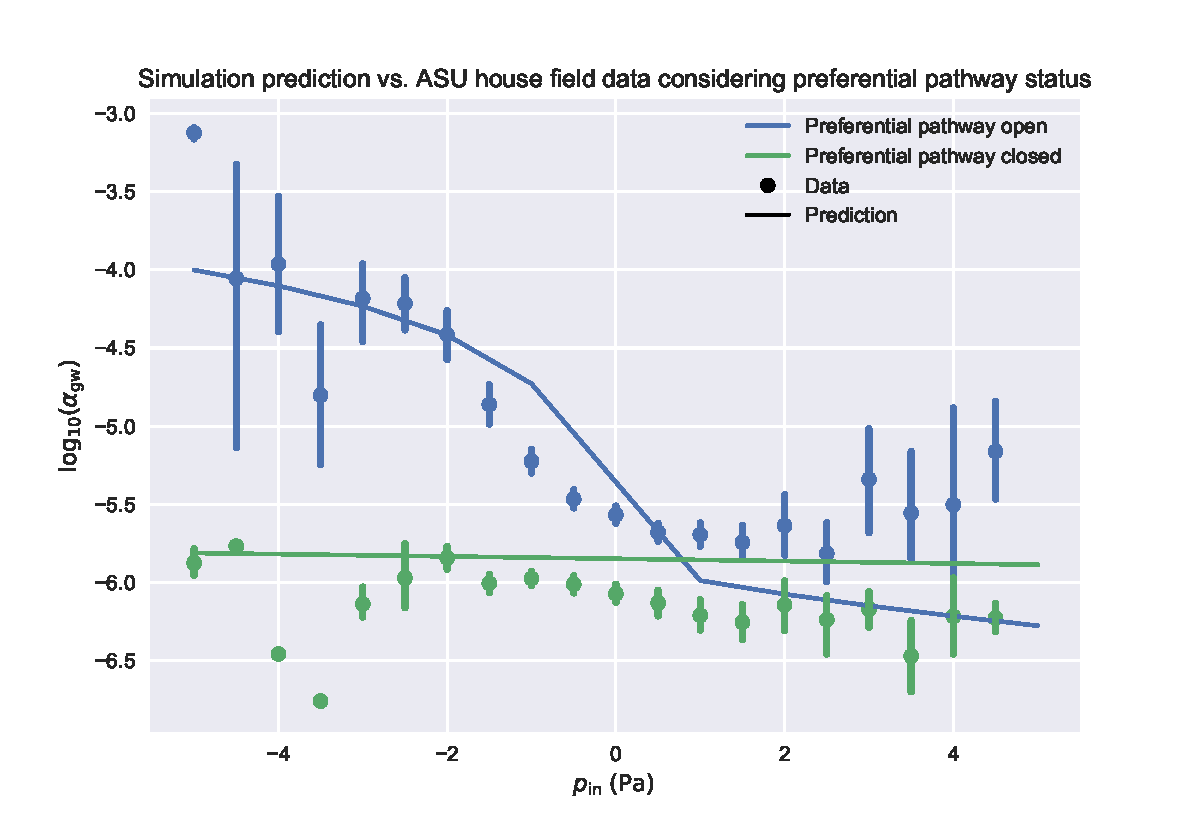
\includegraphics[width=0.85\textwidth]{modeling_results.pdf}
  \caption[Predicted indoor air concentration compared to the ASU house.]{Model predicted indoor air concentration (as groundwater attenuation) compared to values recorded at the ASU house. The modeling results are given the solid lines and data by the dots. Blue here represents data before the closing of the preferential pathway and modeling result from the corresponding model, i.e. the model features a preferential pathway and a gravel sub-base. The green color signifies data from the period after the closing of the preferential pathway with the corresponding model, i.e. the preferential pathway is removed but the gravel sub-base remains. Here the data is placed in 20 equally \textit{spaced bin}, i.e. not equally \textit{sized}. The dot is the mean value and the error bars represent the 95\% confidence intervals.}
  \label{fig:model_results}
\end{figure}

While the intent was not to exactly model all details of the ASU house, the model captures key details such as house footprint size, crack entry size, existence of a gravel sub-base, and a "land drain".
The model successfully predicts the observed trends in $\alpha_\mathrm{gw}$ as $p_\mathrm{in/out}$ decreases (increased depressurization) but somewhat underpredicts $\alpha_\mathrm{gw}$ as the house is overpressurized.
Most significantly, the model captures that even for a small increase in depressurization (0 to -5 Pa) a very large increase in $\alpha_\mathrm{gw}$ (two order of magnitude) can occur.\par

The model is also able to capture the weak trend in $\alpha_\mathrm{gw}$ with $p_\mathrm{in/out}$ when a preferential pathway is absent, but when there still exists a permeable subslab region.
These results are given by the green line in Figure \ref{fig:model_results}.  
These results are again in agreement with what was observed at the ASU House when the preferential pathway was closed, i.e. that there was a much more modest variation in indoor air concentration, irrespective of pressure, when the preferential pathway was cut off.\par

The model corroborates the significant contribution that such a preferential pathway may have at a VI site.
The preferential pathway acts not only as a source of contaminant vapor, but also  as a source of air to the subslab.
Because of the large resistance to soil gas flow in the surrounding soil, having a local source of air to support the increase of advective flow into the structure from the subslab region makes a large difference.
(This will be examined below).
While there obviously is still some variability unaccounted for, as indicated by the error bars on the actual field data in Figure \ref{fig:model_results}, we can say with some confidence that the model is able to capture the general influence of a preferential pathway.
This invites us exploring some of the factors that help explore more of the variability.
Using our model, we rerun the scenarios, but this time consider two more cases:
\begin{enumerate}
  \item We remove the gravel sub-base layer but keep the preferential pathway.
  \item We keep the gravel sub-base layer, but remove contaminant vapor from the preferential pathway, i.e. it supplies only "clean" air.
\end{enumerate}
The results of running these cases can be seen in Figure \ref{fig:model_cases}.\par

\begin{figure}[htb!]
  \centering
  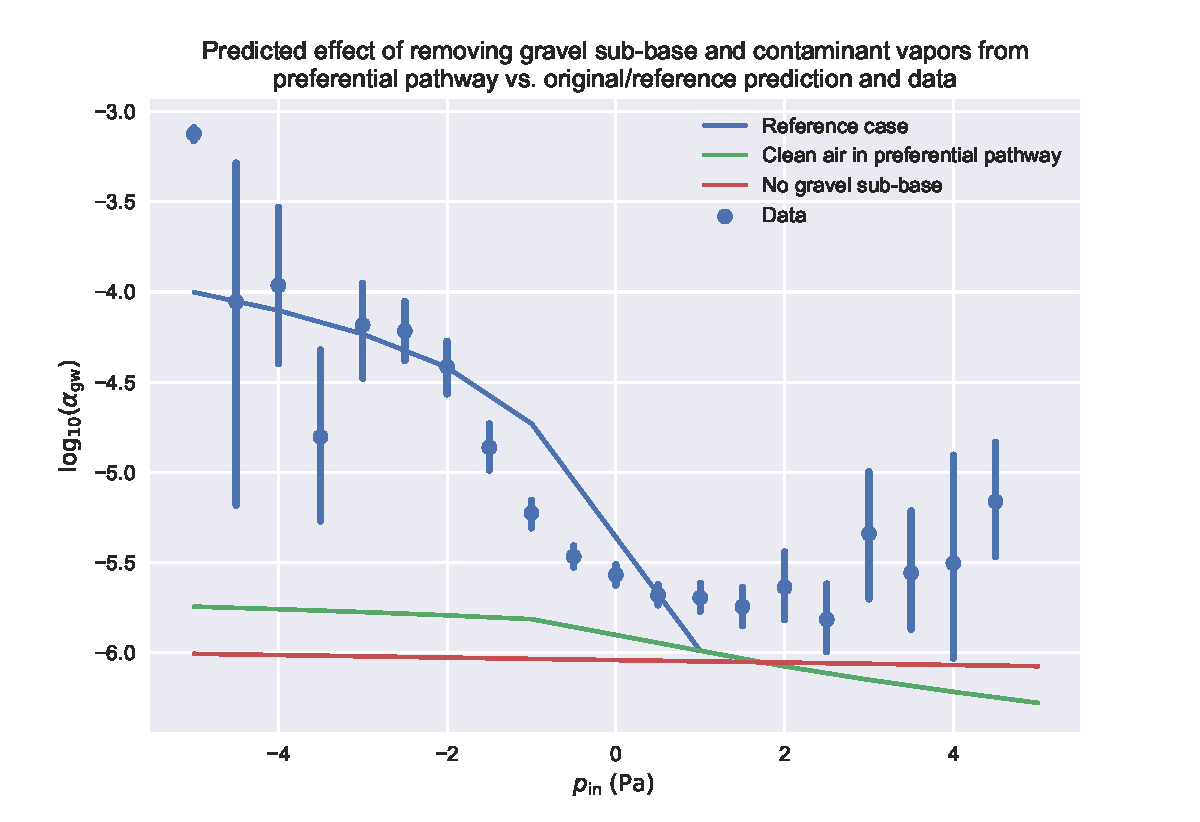
\includegraphics[width=0.85\textwidth]{modeling_cases.pdf}
  \caption{How different cases affect the predicted impact of the preferential pathway.}
  \label{fig:model_cases}
\end{figure}

Here the original modeling results and associated data from the period before the closing of the preferential pathway are again given by blue points and curve.
The case corresponding to the removal of contaminant vapors from the preferential pathway is shown by the green line, while the removal of the gravel sub-base care is shown by red.\par

The removal of contaminant vapors from the preferential pathway largely eliminates the significant dependence of $\alpha_\mathrm{gw}$ on $p_\mathrm{in}$ as shown earlier by blue in Figure \ref{fig:model_results} (see the green curve).
However, the increase in indoor air concentration with decreased indoor pressure is smaller than when the preferential pathway was present.
This shows that a preferential pathway similar to the one found at the ASU house does two things.\par

First, it provides a preferential source of air, and the depressurized building is able to much easier draw air from the preferential pathway than the surrounding soil; the soil offers a huge resistance to airflow and thus advective transport critical to contaminant entry.
Second, the increase in "advective potential" alone is inadequate to cause the large effect as observed at the ASU house, and a preferential source of contaminant vapors is also required - two conditions that were fulfilled at the ASU house.\par

The removal of the gravel sub-base likewise also has a significant effect on the modeling results.
Without it the full potential of a preferential pathway is unrealized (see the red curve).
This can again be understood because of the significant resistance to contaminant transport that soils present.
This adds a third condition for a preferential pathway to exert a significant influence - a medium for effective communication between the preferential pathway and indoor environment is necessary.\par

The importance of advective transport can be shown by analyzing the Péclet number for transport through the foundation crack.
The Péclet number is a dimensionless number defined as the ratio of advective to diffusive transport rate across some characteristic length, i.e. it tell us if transport is advective or diffusion dominated.
For transport of contaminants through the foundation crack we define this as
\begin{equation}\label{eq:peclet_number}
  \mathrm{Pe} = \frac{\mathrm{advection}}{\mathrm{diffusion}} = \frac{u_\mathrm{ck} L_\mathrm{slab}}{D_\mathrm{g}}
\end{equation}
here $u_\mathrm{ck}$ [\si{\metre\per\second}] is the airflow velocity across (through) the crack
$L_\mathrm{slab} = \SI{15}{\centi\metre}$ is the thickness of the foundation slab, i.e. the characteristic length for transport;
and $D_g = \SI{6.87e-6}{\metre\squared\per\second}$ is the diffusivity of TCE in air.\par

\begin{figure}[htb!]
  \centering
  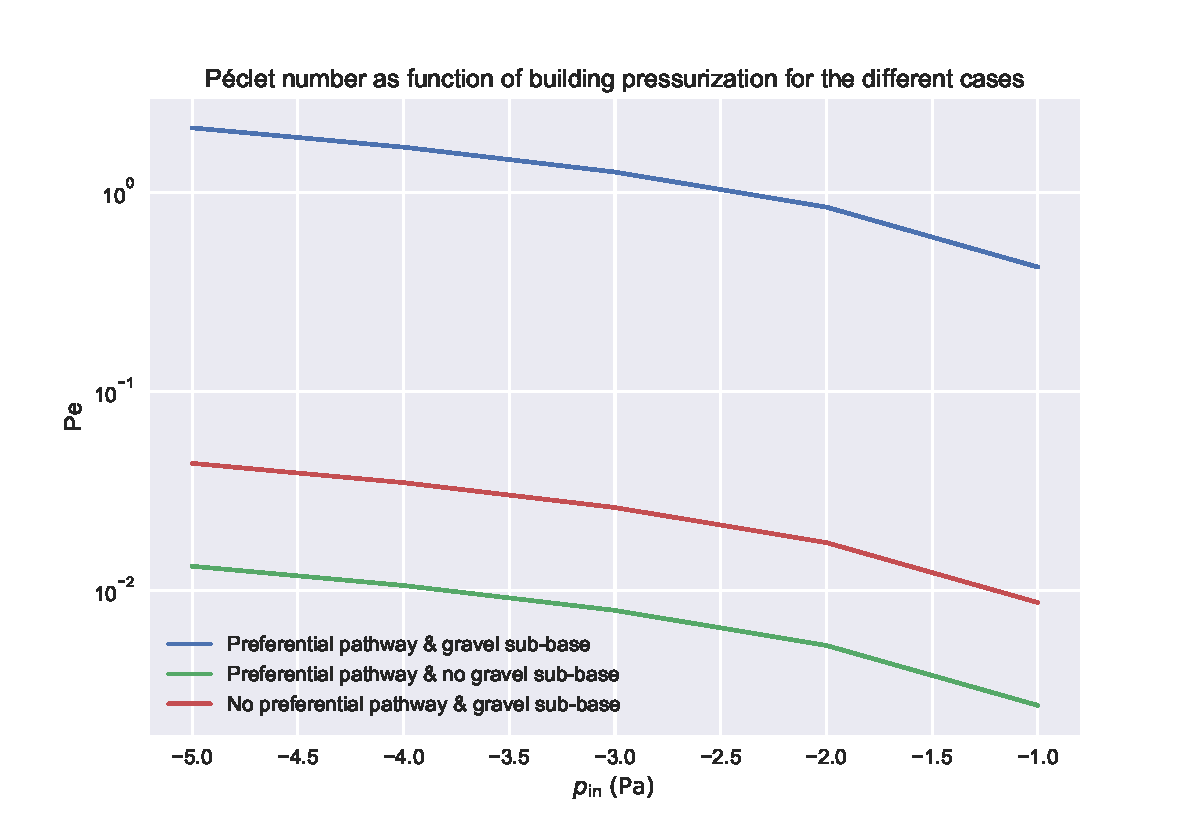
\includegraphics[width=0.85\textwidth]{modeling_result_peclet.pdf}
  \caption[Péclet number for transport through the modeled foundation crack.]{Péclet number for transport through the foundation crack of our modeled house as a fucntion of building pressurization. Here we consider three cases where the preferential pathway and gravel sub-base are present/absent, which shows the dramatic effect these site features can have on contaminant transport at a VI site.}
  \label{fig:peclet_number}
\end{figure}

The values of $\mathrm{Pe}$ characterize transport as:
\begin{align*}
  &\mathrm{Pe} \gg 1 & \text{Advection dominated} \\
  &\mathrm{Pe} \ll 1 & \text{Diffusion dominated} \\
  &\mathrm{Pe} = 1 & \text{Advection and diffusion equal}
\end{align*}
Figure \ref{fig:peclet_number} shows the Péclet number for three of the modeled cases:
\begin{enumerate}
  \item Preferential pathway and gravel sub-base layer present
  \item Preferential pathway present but gravel sub-base layer absent
  \item Preferential pathway absent but gravel sub-base layer present
\end{enumerate}
Note that the cases when $p_\mathrm{in} > \SI{0}{\pascal}$ are not shown.
By our definition $u_\mathrm{ck} > 0$ indicates airflow into the house, giving $\mathrm{Pe} > 0$.
This figure shows that it is only when there is a combination of a preferential pathway and a gravel sub-base layer that advective transport is able to dominate; diffusive transport dominates for the other cases which explains the weak correlation between $\alpha_\mathrm{gw}$ and $p_\mathrm{in}$ in Figure \ref{fig:model_cases} when the preferential pathway was removed.
The rate of diffusion of TCE in air does not depend upon $p_\mathrm{in}$.
Likewise it explains the dramatic increase of $\alpha_\mathrm{gw}$ as $p_\mathrm{in}$ decreases when the  gravel sub-base and preferential pathway were present, as advective transport only starts to dominate after $p_\mathrm{in} < \SI{-2.5}{\pascal}$.\par

To summarize, for a preferential pathway to have a significant influence at a VI site, the following conditions need to be fulfilled:
\begin{enumerate}
  \item A preferential source of air in required to enhance the advective transport potential at the site.
  \item Contaminant vapors must likewise be preferentially supplied.
  \item There needs to exist a medium to facilitate effective communication between the preferential pathway and the indoor environment.
\end{enumerate}
While this may seem like some specific conditions to be fulfilled for a preferential pathway to be so impactful, it can easily be generalized to other scenarios.
For instance, one could easily imagine a situation where a house has a gravel backfill surrounding it, with some other subsurface source - like a leaky sewer pipe (that does not exit anywhere the building).
Under such a circumstance, one could conceivably observe a similar effect in the indoor contaminant concentration caused by a very different scenario.\par

\subsection{Role Of Air Exchange Rate}

Simulations so far has assumed that the indoor air exchange rate is at a constant \SI{0.5}{\per\hour} irrespective of the house pressurization.
This is not quite realistic, as air exchange rates are constantly fluctuating, and this will have an impact on indoor contaminant concentrations.
To account for this, we rerun our model simulations, but this time assuming different air exchange rate values, and determine if this can capture some more of the observed variability.\par

Ideally, we would wish to be able to determine air exchange rate based on site conditions, and in particular building pressurization.
Determining air exchange rate exactly is difficult, as it is influenced by building pressurization, indoor/outdoor temperature differences, wind, operation of HVAC systems, etc.
This is a topic that will be expanded on in Chapter \ref{chp:transport_implications}.\par

Designed air exchange rates are often legally regulated as part of local building ordinances, and depending on the type of building, its values and bounds are usually more or less known.
Here, we will rerun the model and assume a wide range of constant air exchange rate values.
At the ASU house, air exchange rates were measured using a tracer-gas study, and the the \nth{10}, \nth{50}, and \nth{90} percentile air exchange rate values are shown in Table \ref{tbl:air_exchange_rate}.
Also shown are the corresponding values from the EPA duplex, and those from an independent EPA study that measured air exchange rates nationwide.
Based on this we rerun the model using air exchange values of 0.1, 0.5, and \SI{0.9}{\per\hour}.\par

\begin{table}[htb!]
  \centering
  \begin{tabular}{l c c c}
    \toprule
    & \multicolumn{3}{c}{Percentile} \\
    & \nth{10} & \nth{50} & \nth{90} \\
    \midrule
    EPA study\cite{u.s._epa_exposure_2011,m._d._koontz_estimation_1995} & 0.16-0.2 & 0.35-0.49 & 1.21-1.49 \\
    ASU house\cite{holton_temporal_2013,guo_identification_2015} & 0.21 & 0.43 & 0.78 \\
    EPA duplex\cite{u.s._environmental_protection_agency_assessment_2015} & 0.34 & 0.74 & 1.27 \\
    \bottomrule
  \end{tabular}
  \caption{Air exchange rate values [\si{\per\hour}]}
  \label{tbl:air_exchange_rate}
\end{table}

Figure \ref{fig:model_results_air_exchange_rate} shows the result of incorporating a wider range of air exchange rates when predicting $\alpha_\mathrm{gw}$.
Here the central lines are the result corresponding to $A_e = \SI{0.5}{\per\hour}$, while the upper and lower bounds of each shaded area correspond to $A_e = 0.1$ and \SI{0.9}{\per\hour} respectively.
The shaded area cover much of the confidence interval of $\alpha_\mathrm{gw}$ as a function of $p_\mathrm{in}$
This indicates that much of the uncertainty of numerically determining $\alpha_\mathrm{gw}$ could be accounted for by considering the range of air exchange values at a site.\par

\begin{figure}[htb!]
  \centering
  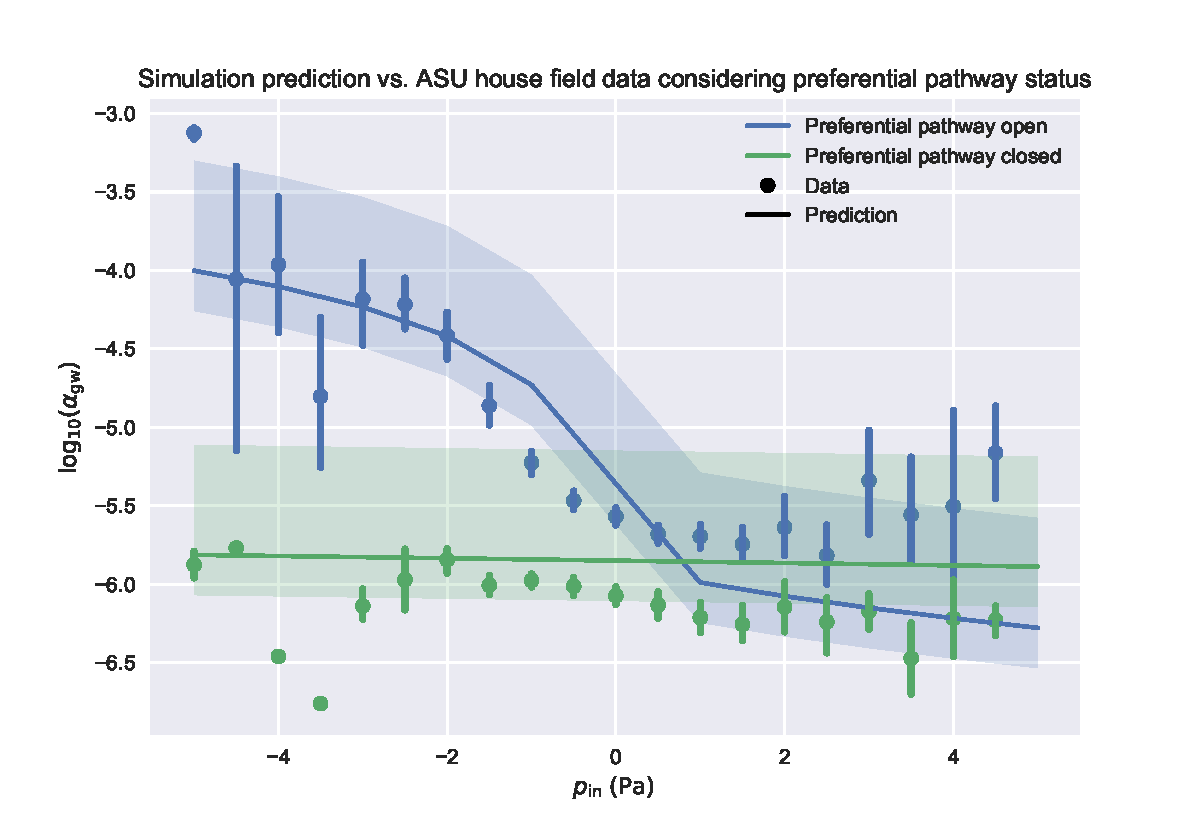
\includegraphics[width=0.85\textwidth]{modeling_result_air_exchange_rate.pdf}
  \caption[Effect of different air exchange rate on predicted indoor contaminant concentration.]{Modeling result from Figure \ref{fig:model_results} but with added shaded area to demonstrate the effect of assuming different air exchange values. The central lines are the result corresponding to $A_e = \SI{0.5}{\per\hour}$, while the upper and lower bounds of each shaded area correspond to $A_e = 0.1$ and \SI{0.9}{\per\hour} respectively.}
  \label{fig:model_results_air_exchange_rate}
\end{figure}

The fact that indoor air pressure and air exchange rate can both vary is applied to a transient simulation, where we model a "typical" day at the ASU house by using the median diurnal variation of $p_\mathrm{in}$ and $A_e$ as model inputs.
We consider our model with and without the preferential pathway present.
Specifically, we use the median diurnal values of $p_\mathrm{in}$ and $A_e$ at one hour intervals over a 24-hour period and interpolate using cubic splines between these for continuity.
This is compared to a case where we only use the median diurnal values of $p_\mathrm{in}$ but keep $A = \SI{0.5}{\per\hour}$ constant.
Now the transient terms neglected at steady-state will be included.\par

Figure \ref{fig:model_diurnal} shows how $\alpha_\mathrm{gw}$ varies throughout this hypothetical "typical" day.
Here we see that when the preferential pathway is present, variability of $\alpha_\mathrm{gw}$ is mostly driven by fluctuations in contaminant entry rate; the variable and constant air exchange rate cases do not differ much from each other.
When the preferential pathway is absent, then there is no variability of $\alpha_\mathrm{gw}$ unless the air exchange rate is fluctuating.\par

\begin{figure}[htb!]
  \centering
  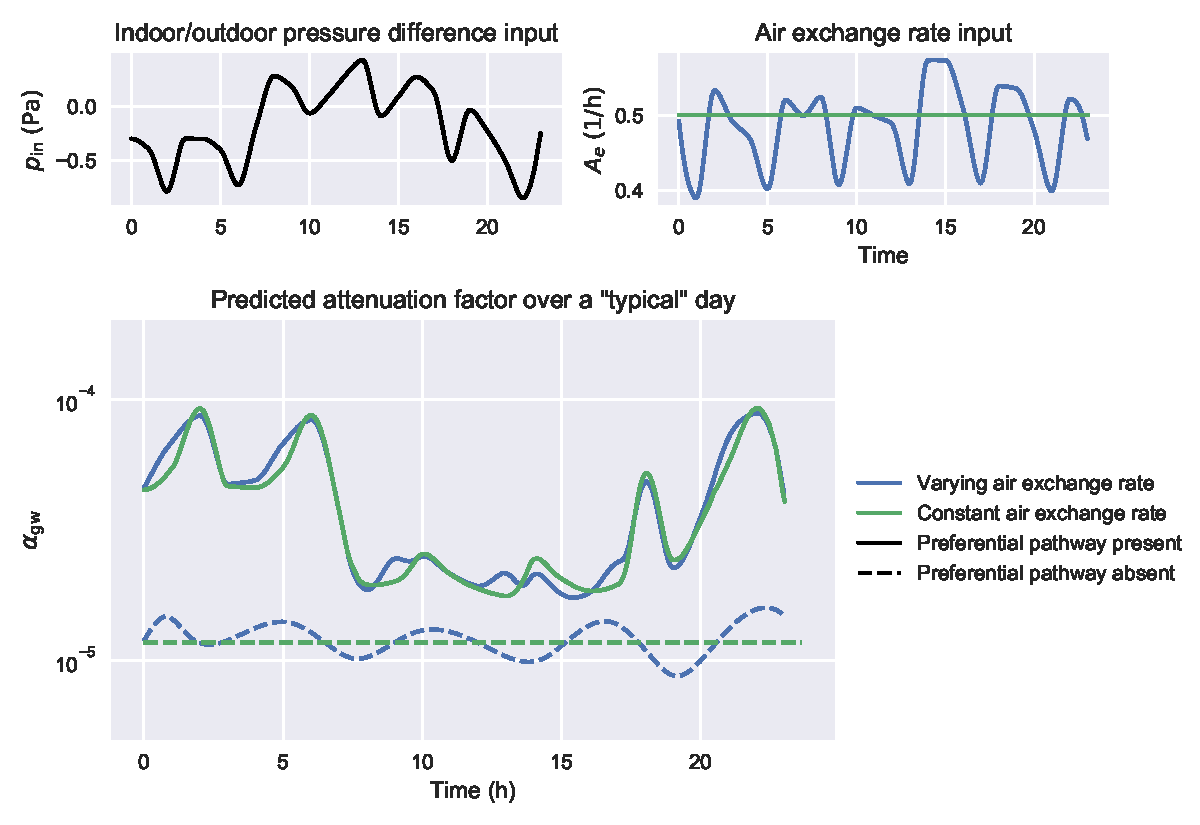
\includegraphics[width=\textwidth]{modeling_diurnal.pdf}
  \caption[Predicted indoor contaminant concentration using diurnal building pressurization and air exchange rates as inputs.]{Modeled indoor contaminant concentration (as attenuation from groundwater) over a "typical" day. Here the hourly median indoor/outdoor pressure difference and air exchange rates recorded at the ASU house, as well as a comparison case where a constant air exchange rate of \SI{0.5}{\per\hour} is assumed, are used as model input parameters. For these we consider two models cases; one where a preferential pathway is present, and another in which it is absent respectively.}
  \label{fig:model_diurnal}
\end{figure}

To quantify the predicted variability of $\alpha_\mathrm{gw}$ we define ratio between the minimum and maximum $\alpha_\mathrm{gw}$ as
\begin{equation}
  \Delta_\mathrm{max} = \frac{\alpha_\mathrm{gw,max}}{\alpha_\mathrm{gw,min}}
\end{equation}
Applying this to the cases where air exchange rate is varied, and the preferential pathway present/absent we find that these ratios are $\Delta_\mathrm{max} = 5.09$ and $\Delta_\mathrm{max} = 1.68$ respectively.
I.e. $\alpha_\mathrm{gw}$ may be expected to vary around half an order of magnitude at a site characterized by a preferential pathway under our considered conditions, whereas one where there is no preferential pathway may vary by a factor of 1.68.\par

These "maximum daily variability" $\Delta_\mathrm{max}$ values can be compared to those at the ASU house.
Indoor contaminant concentration samples at the ASU house were collected roughly every four hours across the study period.
By excluding the CPM period, and then resampling these data on a daily basis, we can find $\Delta_\mathrm{max}$ for each day.
These data are further separated to consider the period before and after the land drain preferential pathway was closed.
The period before the preferential pathway was closed then includes 441 days or data points, giving a median value $\Delta_\mathrm{max} = 2.33$.
For the period after the preferential pathway was closed, we get 181 days of data, giving a median value of $\Delta_\mathrm{max} = 1.60$.
Thus, we can see that we somewhat overpredicted the expected variability for the period when the preferential pathway was open, but were quite close when it was closed.\par

This indicates that for sites that are characterized by diffusive transport, much of the observed variability of indoor contaminant concentrations are driven by fluctuations in air exchange rate.
For sites dominated by advective transport, fluctuations in building pressurization, and consequently contaminant entry, are more important drivers for temporal variability of $\alpha_\mathrm{gw}$.\par
